\documentclass{../../../oss-apphys-exam}
\usepackage{bm}
\usepackage{enumitem}
\newcounter{last}

\runningheader{
  \fontfamily{phv}\small
  \textcolor{gray}{AP PHYSICS C: ELECTRICITY AND MAGNETISM $\blacksquare$}
  \textbf{MULTIPLE-CHOICE QUESTIONS}}{}{}

\begin{document}
%\genheader

\gentitle{14}{HALL EFFECT AND MAXWELL'S EQUATIONS}


\begin{center}
  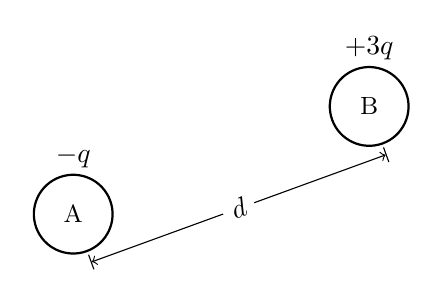
\begin{tikzpicture}[rotate=20]
    \draw[thick] circle (.5) node{\small A} node[above=13]{$-q$};
    \draw[thick] (4,0) circle (.5) node{\small B} node[above=13]{$+3q$};
    \draw[|<->|] (0,-.65)--+(4,0) node[midway,fill=white,rotate=20]{$d$};
  \end{tikzpicture}
\end{center}

\begin{questions}
  \question Conducting spheres A and B of charges $-q$ and $+3q$, respectively,
  are separated by a distance $d$, as shown in the figure above. Which of the
  following statements is true about the two spheres?
  \begin{choices}
    \choice The magnitude of the force sphere A exerts on sphere B is three
    times larger than the magnitude of the force sphere B exerts on sphere A.
    \choice The magnitude of the force sphere B exerts on sphere A is three
    times larger than the magnitude of the force sphere A exerts on sphere B.
    \choice The force sphere B exerts on sphere A is equal in magnitude to the
    force sphere A exerts on sphere B.
    \choice If the spheres are free to move, the magnitude of the force sphere
    B exerts on sphere A will decrease as the spheres move.
    \choice If the spheres are brought into contact with each other and then
    returned to the positions shown, the two spheres will attract each other.
  \end{choices}

  \question Which of the following must be true for a Gaussian surface through
  which the net flux is zero?
  \begin{enumerate}[label={\Roman*.},nosep]
  \item There are no charges inside the surface.
  \item The net charge enclosed by the surface is zero.
  \item The electric field is zero everywhere on the surface.
  \end{enumerate}
  \begin{choices}
    \choice I only
    \choice II only
    \choice III only
    \choice I and II only
    \choice I, II, and III
  \end{choices}
  \uplevel{
    \centering
    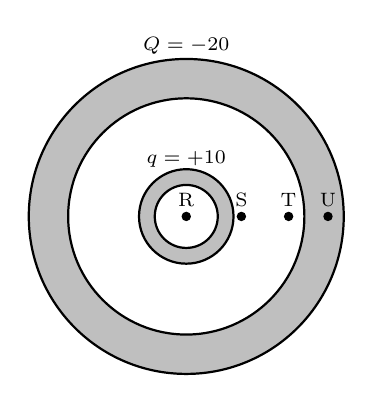
\begin{tikzpicture}
      \draw[thick,fill=lightgray] circle (2) node[above=55]{\scriptsize
        $Q=-\SI{20}{\nano\coulomb}$};
      \draw[thick,fill=white] circle (1.5);
      \draw[thick,fill=lightgray] circle (.6) node[above=14]{\scriptsize
        $q=+\SI{10}{\nano\coulomb}$};
      \draw[thick,fill=white] circle (.4);
      \fill circle (.06) node[above]{\scriptsize R};
      \fill (.7,0) circle (.06) node[above]{\scriptsize S};
      \fill (1.3,0) circle (.06) node[above]{\scriptsize T};
      \fill (1.8,0) circle (.06) node[above]{\scriptsize U};
    \end{tikzpicture}
  }
  \question Two concentric spherical conducting shells and four labeled points
  are shown above. The outer shell has a net charge $Q=-\SI{20}{\nano\coulomb}$.
  The inner shell has a net charge $q=+\SI{10}{\nano\coulomb}$. The magnitudes
  of the electric fields at the four labeled points in the figure are $E_R$,
  $E_S$, $E_T$ and $E_U$, respectively. Which of the following correctly ranks
  the points according to the magnitude of their electric fields?
  \begin{choices}
    \choice $E_R=E_S=E_T=E_U$ 
    \choice $E_S>E_T>(E_R=E_U)$
    \choice $(E_S=E_T)>E_U=E_R$
    \choice $E_T>E_S>E_R=E_U$
    \choice $(E_S=E_T)>(E_R=E_U)$ 
  \end{choices}
  \newpage

  \question An uncharged parallel-plate capacitor is connected through an open
  switch to a battery of voltage $\mathcal E$. The switch is closed and the
  capacitor is allowed to charge. As the capacitor is charged, energy is
  transferred to it from the battery. When the capacitor is fully charged, the
  energy stored in the capacitor is $U_1$. The energy stored in the capacitor
  when the stored charge is $q_0/2$ is
  \begin{choices}
    \choice $\frac14 U_1$
    \choice $\frac12 U_1$
    \choice $U_1$
    \choice $2U_1$
    \choice $4U_1$
  \end{choices}

  \uplevel{
    \centering
    \begin{tikzpicture}
      \foreach \x in {0,.5,...,4}{
        \foreach \y in {-2,-1.5,...,2} \node[gray] at (\x,\y){$\bm\times$};
      }
      \draw[vectors](-1.5,0)--+(1,0) node[above]{$\vec v$};
      \draw[thick,fill=white] (-1.5,0) circle (.15) node{\scriptsize $\bm-$}
       node[left=4]{\scriptsize Electron};
      \draw[vectors,rotate=45] (0,0) --+(1.5,0) node[above]{A};
      \draw[vectors] (0,0) arc (270:330:1.5) node[right]{B};
      \draw[vectors] (0,0)--+(1.5,0) node[right]{C};
      \draw[vectors] (0,0) arc (90:30:1.5) node[right]{D};
      \draw[vectors,rotate=-45] (0,0) --+(1.5,0) node[below]{E};
    \end{tikzpicture}
  }
  \question An electron is traveling with velocity $\vec v$ when it enters a
  uniform magnetic field $\vec B$ directed into the page, as shown above. Five
  paths in the magnetic field are labeled A, B, C, D, and E. Which labeled path
  best shows the path the electron will follow as it travels through the
  magnetic field?
  \begin{choices}
    \choice Path A
    \choice Path B
    \choice Path C
    \choice Path D
    \choice Path E
  \end{choices}

  \question A loop of wire with resistance \SI2{\ohm} lies in a magnetic field.
  The magnetic flux $\phi_m$ through the loop as a function of time $t$ is given
  by $\phi_m=(2t^2+2t)$, where $\phi_m$ is in \si{\tesla.\meter\squared} and $t$
  is in seconds. What is the current in the loop at $t=\SI3\second$?
  \begin{choices}
    \choice 6 A 
    \choice 7 A 
    \choice 12 A
    \choice 14 A
    \choice 24 A
  \end{choices}
\end{questions}
\setcounter{last}{\value{question}}
\newpage
  
\runningheader{
  \fontfamily{phv}\small
  \textcolor{gray}{AP PHYSICS C: ELECTRICITY AND MAGNETISM $\blacksquare$}
  \textbf{FREE-RESPONSE QUESTIONS}}{}{}
  
% TAKEN FROM THE 2009 AP PHYSICS C FREE-RESPONSE QUESTION E&M 2. THIS IS A
% HALL-EFFECT QUESTION
\begin{center}
  \pic{.45}{hall2}
\end{center}

\begin{questions}
  \setcounter{question}{\value{last}}
  
  \question A \SI{9.0}{\volt} battery is connected to a rectangular bar of
  length \SI{0.080}{\metre}, uniform cross-sectional area
  \SI{5.0e-6}{\metre\squared}, and resistivity \SI{4.5e-4}{\ohm\metre}, as
  shown above. Electrons are the sole charge carriers in the bar. The wires
  have negligible resistance. The switch in the circuit is closed at time $t=0$.

  \begin{parts}
    \part\textbf{Calculate} the power delivered to the circuit by the battery.
    \vspace{\stretch1}
    
    \part On the diagram below, \textbf{indicate} the direction of the electric
    field in the bar.
    \begin{center}
      \vspace{.2in}
      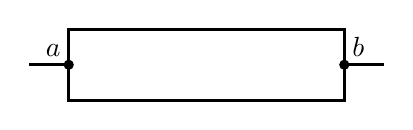
\begin{tikzpicture}[scale=.5,very thick]
        \draw (.5,.6) rectangle (7.5,2.4);
        \draw (-.5,1.5)--(.5,1.5);
        \draw (7.5,1.5)--(8.5,1.5);
        \fill (.5,1.5) circle (.13) node[above left=-1]{$a$};
        \fill (7.5,1.5) circle (.13) node[above right=-1]{$b$};
      \end{tikzpicture}\\
      Side View
      \vspace{.2in}
    \end{center}
    \textbf{Explain} your answer.
    \vspace{\stretch1}
    
    \part\textbf{Calculate} the magnitude of the electric field in the bar.
    \vspace{\stretch1}
    \newpage
    
    \uplevel{
      A uniform magnetic field of magnitude \SI{.25}{\tesla} perpendicular to
      the bar is added to the region around the bar, as shown below.
      \cpic{.8}{hall1}
    }

    \part\textbf{Calculate} the magnitude of the magnetic force on the bar.
    \vspace{\stretch1}
    
    \part The electrons moving through the bar are initially deflected by the
    external magnetic field. On the diagram below, indicate the direction of
    the additional electric field that is created in the bar by the deflected
    electrons.
    \begin{center}
      \vspace{.1in}
      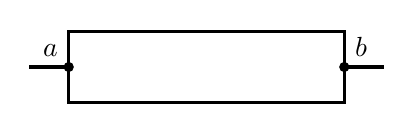
\begin{tikzpicture}[scale=.5, very thick]
        \draw (.5,.6) rectangle (7.5,2.4);
        \draw (-.5,1.5)--(.5,1.5);
        \draw (7.5,1.5)--(8.5,1.5);
        \fill (.5,1.5) circle (.13) node[above left]{$a$};
        \fill (7.5,1.5) circle (.13) node[above right]{$b$};
      \end{tikzpicture}\\
      Side View
      \vspace{.1in}
    \end{center}

    \part The electrons eventually experience no deflection and move through the
    bar at an average speed of \SI{3.5e-3}{\metre\per\second}.
    \textbf{Calculate} the strength of the additional electric field indicated
    in part \textbf{E}.
    \vspace{\stretch2}        
  \end{parts}
  \newpage

  % TAKEN FROM THE 2009 AP PHYSICS C EXAM FREE-RESPONSE QUESTION E&M 3
  % THIS IS A QUESTION ON MAGNETIC INDUCTION
  \uplevel{
    \centering
    \begin{tikzpicture}[scale=.8]
      \foreach\x in {0,...,3}{
        \foreach\y in {0,...,3} \node[gray] at (\x,\y){$\bm\times$};
      }
      \draw[thick] (-.5,-.5) to[rmeter,t=1](-.5,3.5)--(3.5,3.5)
      to[rmeter,t=2] (3.5,-.5)--(-.5,-.5);
      \node at (1.5,1.5){$B$};
      \draw[thick,|<->|] (-.5,3.85)--(3.5,3.85) node[midway,fill=white]{$L$};
    \end{tikzpicture}
  }
  
  \question A square conducting loop of side $L$ contains two identical
  lightbulbs, 1 and 2, as shown above. There is a magnetic field directed into
  the page in the region inside the loop with magnitude as a function of time
  $t$ given by $B(t)=at+b$, where $a$ and $b$ are positive constants. The
  lightbulbs each have constant resistance $R_0$. Express all answers in terms
  of the given quantities and fundamental constants.
  \begin{parts}
    \part\textbf{Derive} an expression for the magnitude of the \emph{emf}
    generated in the loop.
    \vspace{\stretch1}
    
    \part\textbf{Determine} an expression for the current through bulb 2.
    \vspace{\stretch1}

    \part\textbf{Indicate} on the diagram above the direction of the current
    through bulb 2. \textbf{Explain} your answer.
    \vspace{\stretch1}
    
    \part\textbf{Derive} an expression for the power dissipated in bulb 1.
    \vspace{\stretch1}
    
    \uplevel{
      Another identical bulb 3 is now connected in parallel with bulb 2, but it
      is entirely outside the magnetic field, as shown below.
      \begin{center}
        \begin{tikzpicture}[scale=.8]
          \foreach \x in {0,...,3}{
            \foreach \y in {0,...,3} \node[gray] at (\x,\y){$\bm\times$};
          }
          \draw[thick] (-.5,-.5) to[rmeter,t=1](-.5,3.5)--(3.5,3.5)
          to[rmeter,t=2] (3.5,-.5)--(-.5,-.5);
          \draw[thick] (3.5,3.5)--(5.5,3.5) to[rmeter,t=3](5.5,-.5)--(3.5,-.5);
          \node at (1.5,1.5){$B$};
          \draw[thick,|<->|] (-.5,3.9)--(3.5,3.9) node[midway,fill=white]{$L$};
        \end{tikzpicture}
      \end{center}
    }

    \part How does the brightness of bulb 1 compare to what it was in the
    previous circuit?

    \vspace{.1in}
    \underline{\hspace{.3in}} Brighter\hspace{.5in}
    \underline{\hspace{.3in}} Dimmer\hspace{.5in}
    \underline{\hspace{.3in}} The same

    \vspace{.15in}\textbf{Justify} your answer.
    \vspace{\stretch1}
    \newpage
    
    \uplevel{
      Now the portion of the circuit containing bulb 3 is removed, and a wire is
      added to connect the midpoints of the top and bottom of the original
      loop, as shown below.
      \begin{center}
        \begin{tikzpicture}[scale=.8]
          \foreach \x in {0,...,3}{
            \foreach \y in {0,...,3} \node[gray] at (\x,\y){$\bm\times$};
          }
          \draw[thick] (-.5,-.5) to[rmeter,t=1](-.5,3.5)--(3.5,3.5)
          to[rmeter,t=2] (3.5,-.5)--(-.5,-.5);
          \draw[thick] (1.5,3.5)--(1.5,-.5);
          \node at (.5,1.5){$B$};
          \node at (2.5,1.5){$B$};
          \draw[thick,|<->|] (-.5,3.9)--(3.5,3.9) node[midway,fill=white]{$L$};
        \end{tikzpicture}
      \end{center}
    }

    \part How does the brightness of bulb 1 compare to what it was in the first
    circuit?

    \vspace{.1in}
    \underline{\hspace{.3in}} Brighter\hspace{.5in}
    \underline{\hspace{.3in}} Dimmer\hspace{.5in}
    \underline{\hspace{.3in}} The same
  \end{parts}

  \vspace{.15in}\textbf{Justify} your answer.
  \newpage

  \uplevel{
    \centering
    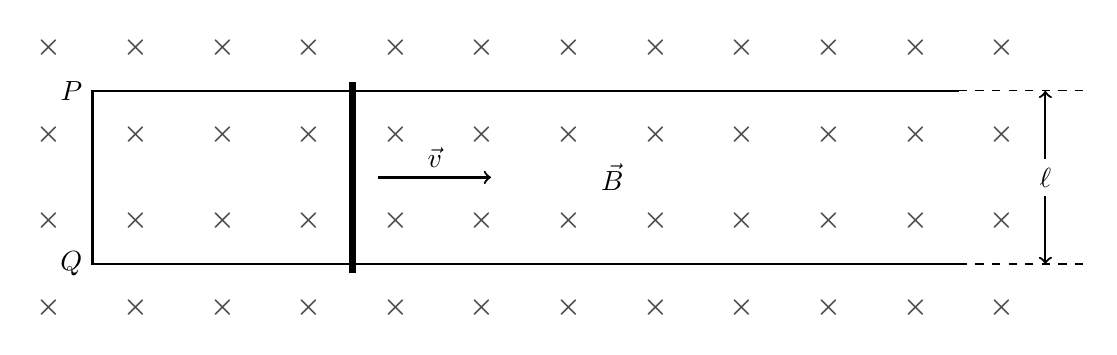
\begin{tikzpicture}[scale=1.1]
      \foreach \x in {0,...,11}
      \foreach \y in {0,...,3} \node[black!70] at (\x,\y) {$\bm\times$};
      \draw[thick] (10.5,.5)--(.5,.5) node[left]{$Q$}--(.5,2.5) node[left]{$P$}
      --(10.5,2.5);
      \draw[dashed] (10.5,2.5)--(12,2.5);
      \draw[dashed] (10.5,0.5)--(12,0.5);
      \draw[line width=2.3] (3.5,.4)--(3.5,2.6);
      \node at (6.5,1.5) {$\vec B$};
      \draw[thick,<->] (11.5,.5)--(11.5,2.5) node[midway,fill=white]{$\ell$};
      \draw[thick,->] (3.8,1.5)--(5.1,1.5) node[midway,above]{$\vec v$};
    \end{tikzpicture}\\
    Top View
  }
  
  \question In the diagram above, a nichrome wire of resistance per unit length
  $\lambda$ is bent at points $P$ and $Q$ to form horizontal conducting rails
  that are a distance $\ell$ apart. The wire is placed within a uniform
  magnetic field $B$ pointing into the page. A conducting rod of negligible
  resistance, which was aligned with end $PQ$ at time $t=0$, slides to the
  right with constant velocity $\vec v$ and negligible friction. Express all
  algebraic answers in terms of the given quantities and fundamental constants.
  \begin{parts}
    \part\textbf{Indicate} the direction of the current induced in the circuit.

    \vspace{.1in}
    \underline{\hspace{.3in}} Clockwise\hspace{.5in}
    \underline{\hspace{.3in}} Counterclockwise

    \vspace{.1in}\textbf{Justify} your answer.
    \vspace{\stretch1}
    
    \part\textbf{Derive} an expression for the magnitude of the induced current
    $I$ as a function of time $t$.
    \vspace{\stretch1}
    
    \part\textbf{Derive} an expression for the magnitude of the magnetic force
    $F_m$ on the rod as a function of time $t$.
    \vspace{\stretch1}
    
    \part On the axes below, \textbf{sketch} a graph of the external force
    $F_\text{ext}$ as a function of time that must be applied to the rod to keep
    it moving at constant speed while in the field. \textbf{Label} the values
    of any intercepts.
    \begin{center}
      \begin{tikzpicture}
        \draw[axes] (0,0)--(7,0) node[right]{$t$} node[pos=0,below left]{$O$};
        \draw[axes] (0,0)--(0,4) node[above]{$F_\text{ext}$};
      \end{tikzpicture}
    \end{center}
    \newpage
    
    \part The force pulling the rod is now removed. \textbf{Indicate} whether
    the speed of the rod increases, decreases, or remains the same.

    \vspace{.1in}
    \underline{\hspace{.3in}} Increases\hspace{.5in}
    \underline{\hspace{.3in}} Decreases\hspace{.5in}
    \underline{\hspace{.3in}} Remains the same
    
    \vspace{.15in}\textbf{Justify} your answer.
  \end{parts}
\end{questions}
\end{document}
